% Options for packages loaded elsewhere
% Options for packages loaded elsewhere
\PassOptionsToPackage{unicode}{hyperref}
\PassOptionsToPackage{hyphens}{url}
\PassOptionsToPackage{dvipsnames,svgnames,x11names}{xcolor}
%
\documentclass[
  french,
]{report}
\usepackage{xcolor}
\usepackage{amsmath,amssymb}
\setcounter{secnumdepth}{-\maxdimen} % remove section numbering
\usepackage{iftex}
\ifPDFTeX
  \usepackage[T1]{fontenc}
  \usepackage[utf8]{inputenc}
  \usepackage{textcomp} % provide euro and other symbols
\else % if luatex or xetex
  \usepackage{unicode-math} % this also loads fontspec
  \defaultfontfeatures{Scale=MatchLowercase}
  \defaultfontfeatures[\rmfamily]{Ligatures=TeX,Scale=1}
\fi
\usepackage{lmodern}
\ifPDFTeX\else
  % xetex/luatex font selection
\fi
% Use upquote if available, for straight quotes in verbatim environments
\IfFileExists{upquote.sty}{\usepackage{upquote}}{}
\IfFileExists{microtype.sty}{% use microtype if available
  \usepackage[]{microtype}
  \UseMicrotypeSet[protrusion]{basicmath} % disable protrusion for tt fonts
}{}
\makeatletter
\@ifundefined{KOMAClassName}{% if non-KOMA class
  \IfFileExists{parskip.sty}{%
    \usepackage{parskip}
  }{% else
    \setlength{\parindent}{0pt}
    \setlength{\parskip}{6pt plus 2pt minus 1pt}}
}{% if KOMA class
  \KOMAoptions{parskip=half}}
\makeatother
% Make \paragraph and \subparagraph free-standing
\makeatletter
\ifx\paragraph\undefined\else
  \let\oldparagraph\paragraph
  \renewcommand{\paragraph}{
    \@ifstar
      \xxxParagraphStar
      \xxxParagraphNoStar
  }
  \newcommand{\xxxParagraphStar}[1]{\oldparagraph*{#1}\mbox{}}
  \newcommand{\xxxParagraphNoStar}[1]{\oldparagraph{#1}\mbox{}}
\fi
\ifx\subparagraph\undefined\else
  \let\oldsubparagraph\subparagraph
  \renewcommand{\subparagraph}{
    \@ifstar
      \xxxSubParagraphStar
      \xxxSubParagraphNoStar
  }
  \newcommand{\xxxSubParagraphStar}[1]{\oldsubparagraph*{#1}\mbox{}}
  \newcommand{\xxxSubParagraphNoStar}[1]{\oldsubparagraph{#1}\mbox{}}
\fi
\makeatother


\usepackage{longtable,booktabs,array}
\usepackage{calc} % for calculating minipage widths
% Correct order of tables after \paragraph or \subparagraph
\usepackage{etoolbox}
\makeatletter
\patchcmd\longtable{\par}{\if@noskipsec\mbox{}\fi\par}{}{}
\makeatother
% Allow footnotes in longtable head/foot
\IfFileExists{footnotehyper.sty}{\usepackage{footnotehyper}}{\usepackage{footnote}}
\makesavenoteenv{longtable}
\usepackage{graphicx}
\makeatletter
\newsavebox\pandoc@box
\newcommand*\pandocbounded[1]{% scales image to fit in text height/width
  \sbox\pandoc@box{#1}%
  \Gscale@div\@tempa{\textheight}{\dimexpr\ht\pandoc@box+\dp\pandoc@box\relax}%
  \Gscale@div\@tempb{\linewidth}{\wd\pandoc@box}%
  \ifdim\@tempb\p@<\@tempa\p@\let\@tempa\@tempb\fi% select the smaller of both
  \ifdim\@tempa\p@<\p@\scalebox{\@tempa}{\usebox\pandoc@box}%
  \else\usebox{\pandoc@box}%
  \fi%
}
% Set default figure placement to htbp
\def\fps@figure{htbp}
\makeatother



\ifLuaTeX
\usepackage[bidi=basic]{babel}
\else
\usepackage[bidi=default]{babel}
\fi
% get rid of language-specific shorthands (see #6817):
\let\LanguageShortHands\languageshorthands
\def\languageshorthands#1{}


\setlength{\emergencystretch}{3em} % prevent overfull lines

\providecommand{\tightlist}{%
  \setlength{\itemsep}{0pt}\setlength{\parskip}{0pt}}



 


\usepackage{multirow}
\usepackage{longtable}
\usepackage{caption}
\makeatletter
\@ifpackageloaded{caption}{}{\usepackage{caption}}
\AtBeginDocument{%
\ifdefined\contentsname
  \renewcommand*\contentsname{Table des matières}
\else
  \newcommand\contentsname{Table des matières}
\fi
\ifdefined\listfigurename
  \renewcommand*\listfigurename{Liste des Figures}
\else
  \newcommand\listfigurename{Liste des Figures}
\fi
\ifdefined\listtablename
  \renewcommand*\listtablename{Liste des Tables}
\else
  \newcommand\listtablename{Liste des Tables}
\fi
\ifdefined\figurename
  \renewcommand*\figurename{Figure}
\else
  \newcommand\figurename{Figure}
\fi
\ifdefined\tablename
  \renewcommand*\tablename{Table}
\else
  \newcommand\tablename{Table}
\fi
}
\@ifpackageloaded{float}{}{\usepackage{float}}
\floatstyle{ruled}
\@ifundefined{c@chapter}{\newfloat{codelisting}{h}{lop}}{\newfloat{codelisting}{h}{lop}[chapter]}
\floatname{codelisting}{Listing}
\newcommand*\listoflistings{\listof{codelisting}{Liste des Listings}}
\makeatother
\makeatletter
\makeatother
\makeatletter
\@ifpackageloaded{caption}{}{\usepackage{caption}}
\@ifpackageloaded{subcaption}{}{\usepackage{subcaption}}
\makeatother
\usepackage{bookmark}
\IfFileExists{xurl.sty}{\usepackage{xurl}}{} % add URL line breaks if available
\urlstyle{same}
\hypersetup{
  pdftitle={Test Layout --- Tables et Figures},
  pdflang={fr},
  colorlinks=true,
  linkcolor={blue},
  filecolor={Maroon},
  citecolor={Blue},
  urlcolor={Blue},
  pdfcreator={LaTeX via pandoc}}


\title{Test Layout --- Tables et Figures}
\author{}
\date{}
\begin{document}
\maketitle


\chapter{Test 1: Simple table --- Taille moyenne des
ménages}\label{test-1-simple-table-taille-moyenne-des-muxe9nages}

\begin{longtable}[]{@{}lr@{}}

\caption{\label{tbl-test-simple}}

\tabularnewline

\toprule\noalign{}
Observatoire & Taille moyenne \\
\midrule\noalign{}
\endhead
\midrule\noalign{}
\multicolumn{2}{@{}l@{}}{%
{\textbf{Source : Enquête auprès des OR 2025}}} \\
\bottomrule\noalign{}
\endlastfoot
Alaotra & 3.90 \\
Marovoay & 4.43 \\

\end{longtable}

\chapter{Test 2: Grouped table --- Répartition par tranche
d'âge}\label{test-2-grouped-table-ruxe9partition-par-tranche-duxe2ge}

\begin{longtable}[]{@{}lll@{}}

\caption{\label{tbl-test-grouped}}

\tabularnewline

\toprule\noalign{}
\multicolumn{3}{@{}c@{}}{%
Répartition des membres du ménage par tranche d\textquotesingle âge} \\
Tranche d\textquotesingle âge & Effectif & \% \\
\midrule\noalign{}
\endhead
\midrule\noalign{}
\multicolumn{3}{@{}l@{}}{%
{\textbf{Source : Enquête auprès des OR 2025}}} \\
\bottomrule\noalign{}
\endlastfoot
\multicolumn{3}{@{}l@{}}{%
Alaotra} \\
0-10 ans & 551 & 27.9 \\
11-20 ans & 407 & 20.6 \\
21-30 ans & 322 & 16.3 \\
31-40 ans & 232 & 11.8 \\
41-50 ans & 177 & 9.0 \\
51-60 ans & 143 & 7.2 \\
61-70 ans & 88 & 4.5 \\
71 ans et plus & 53 & 2.7 \\
\multicolumn{3}{@{}l@{}}{%
Marovoay} \\
0-10 ans & 679 & 29.6 \\
11-20 ans & 542 & 23.6 \\
21-30 ans & 355 & 15.5 \\
31-40 ans & 222 & 9.7 \\
41-50 ans & 193 & 8.4 \\
51-60 ans & 146 & 6.4 \\
61-70 ans & 124 & 5.4 \\
71 ans et plus & 36 & 1.6 \\

\end{longtable}

\chapter{Test 3: Wide table --- Éducation CM par sexe (4 obs × sexe
columns)}\label{test-3-wide-table-uxe9ducation-cm-par-sexe-4-obs-sexe-columns}

\begin{longtable}[]{@{}
  >{\raggedright\arraybackslash}p{(\linewidth - 8\tabcolsep) * \real{0.2000}}
  >{\raggedleft\arraybackslash}p{(\linewidth - 8\tabcolsep) * \real{0.2000}}
  >{\raggedleft\arraybackslash}p{(\linewidth - 8\tabcolsep) * \real{0.2000}}
  >{\raggedleft\arraybackslash}p{(\linewidth - 8\tabcolsep) * \real{0.2000}}
  >{\raggedleft\arraybackslash}p{(\linewidth - 8\tabcolsep) * \real{0.2000}}@{}}

\caption{\label{tbl-test-wide}}

\tabularnewline

\toprule\noalign{}
\multicolumn{5}{@{}>{\centering\arraybackslash}p{(\linewidth - 8\tabcolsep) * \real{1.0000} + 8\tabcolsep}@{}}{%
\begin{minipage}[b]{\linewidth}\centering
Répartition des CM selon le niveau d\textquotesingle éducation et le
sexe{\textsuperscript{1}}
\end{minipage}} \\
\multirow{2}{=}{\begin{minipage}[b]{\linewidth}\raggedright
Niveau d\textquotesingle éducation
\end{minipage}} &
\multicolumn{2}{>{\centering\arraybackslash}p{(\linewidth - 8\tabcolsep) * \real{0.4000} + 2\tabcolsep}}{%
\begin{minipage}[b]{\linewidth}\centering
Alaotra
\end{minipage}} &
\multicolumn{2}{>{\centering\arraybackslash}p{(\linewidth - 8\tabcolsep) * \real{0.4000} + 2\tabcolsep}@{}}{%
\begin{minipage}[b]{\linewidth}\centering
Marovoay
\end{minipage}} \\
& \begin{minipage}[b]{\linewidth}\raggedleft
Homme
\end{minipage} & \begin{minipage}[b]{\linewidth}\raggedleft
Femme
\end{minipage} & \begin{minipage}[b]{\linewidth}\raggedleft
Homme
\end{minipage} & \begin{minipage}[b]{\linewidth}\raggedleft
Femme
\end{minipage} \\
\midrule\noalign{}
\endhead
\midrule\noalign{}
\multicolumn{5}{@{}>{\raggedright\arraybackslash}p{(\linewidth - 8\tabcolsep) * \real{1.0000} + 8\tabcolsep}@{}}{%
{\textsuperscript{1}} Pourcentages calculés par rapport au total des CM
de chaque sexe et observatoire.} \\
\multicolumn{5}{@{}>{\raggedright\arraybackslash}p{(\linewidth - 8\tabcolsep) * \real{1.0000} + 8\tabcolsep}@{}}{%
{\textbf{Source : Enquête auprès des OR 2025}}} \\
\bottomrule\noalign{}
\endlastfoot
Inconnu & 33 (8.3\%) & 18 (16.4\%) & 65 (16\%) & 13 (11.4\%) \\
Primaire & 237 (59.7\%) & 70 (63.6\%) & 199 (49.1\%) & 70 (61.4\%) \\
Secondaire 1er cycle & 92 (23.2\%) & 17 (15.5\%) & 104 (25.7\%) & 26
(22.8\%) \\
Secondaire 2ème cycle \& sup. & 35 (8.8\%) & 5 (4.5\%) & 37 (9.1\%) & 5
(4.4\%) \\

\end{longtable}

\chapter{Test 4: Wide table with spanners --- Activités CM par
sexe}\label{test-4-wide-table-with-spanners-activituxe9s-cm-par-sexe}

\begin{longtable}[]{@{}
  >{\raggedright\arraybackslash}p{(\linewidth - 8\tabcolsep) * \real{0.2000}}
  >{\raggedright\arraybackslash}p{(\linewidth - 8\tabcolsep) * \real{0.2000}}
  >{\raggedright\arraybackslash}p{(\linewidth - 8\tabcolsep) * \real{0.2000}}
  >{\raggedright\arraybackslash}p{(\linewidth - 8\tabcolsep) * \real{0.2000}}
  >{\raggedright\arraybackslash}p{(\linewidth - 8\tabcolsep) * \real{0.2000}}@{}}

\caption{\label{tbl-test-wide-activity}}

\tabularnewline

\toprule\noalign{}
\multicolumn{5}{@{}>{\centering\arraybackslash}p{(\linewidth - 8\tabcolsep) * \real{1.0000} + 8\tabcolsep}@{}}{%
\begin{minipage}[b]{\linewidth}\centering
Activités principales des CM par observatoire et sexe
\end{minipage}} \\
\multirow{2}{=}{\begin{minipage}[b]{\linewidth}\raggedright
Activité
\end{minipage}} &
\multicolumn{2}{>{\centering\arraybackslash}p{(\linewidth - 8\tabcolsep) * \real{0.4000} + 2\tabcolsep}}{%
\begin{minipage}[b]{\linewidth}\centering
Femme
\end{minipage}} &
\multicolumn{2}{>{\centering\arraybackslash}p{(\linewidth - 8\tabcolsep) * \real{0.4000} + 2\tabcolsep}@{}}{%
\begin{minipage}[b]{\linewidth}\centering
Homme
\end{minipage}} \\
& \begin{minipage}[b]{\linewidth}\raggedleft
N
\end{minipage} & \begin{minipage}[b]{\linewidth}\raggedleft
\%
\end{minipage} & \begin{minipage}[b]{\linewidth}\raggedleft
N
\end{minipage} & \begin{minipage}[b]{\linewidth}\raggedleft
\%
\end{minipage} \\
\midrule\noalign{}
\endhead
\midrule\noalign{}
\multicolumn{5}{@{}>{\raggedright\arraybackslash}p{(\linewidth - 8\tabcolsep) * \real{1.0000} + 8\tabcolsep}@{}}{%
{\textbf{Source : Enquête auprès des OR 2025}}} \\
\bottomrule\noalign{}
\endlastfoot
\multicolumn{5}{@{}>{\raggedright\arraybackslash}p{(\linewidth - 8\tabcolsep) * \real{1.0000} + 8\tabcolsep}@{}}{%
Alaotra} \\
Cultivateur exploitant & 46 & 42.2 & 259 & 65.4 \\
Commerce \& Restauration & 18 & 16.5 & 10 & 2.5 \\
Services \& Autres & 18 & 16.5 & 15 & 3.8 \\
Ouvrier agricole & 13 & 11.9 & 50 & 12.6 \\
Artisanat, BTP \& Transport & 8 & 7.3 & 37 & 9.3 \\
Elevage, Pêche \& Ress. nat. & 6 & 5.5 & 25 & 6.3 \\
\multicolumn{5}{@{}>{\raggedright\arraybackslash}p{(\linewidth - 8\tabcolsep) * \real{1.0000} + 8\tabcolsep}@{}}{%
Marovoay} \\
Cultivateur exploitant & 37 & 32.5 & 267 & 65.9 \\
Ouvrier agricole & 35 & 30.7 & 60 & 14.8 \\
Commerce \& Restauration & 26 & 22.8 & 12 & 3.0 \\
Services \& Autres & 8 & 7.0 & 14 & 3.5 \\
Elevage, Pêche \& Ress. nat. & 5 & 4.4 & 20 & 4.9 \\
Artisanat, BTP \& Transport & \textless{} 5 & \textless{} 5 & 32 &
7.9 \\

\end{longtable}

\chapter{Test 5: Homeland table (very
wide)}\label{test-5-homeland-table-very-wide}

\begin{longtable}[]{@{}
  >{\raggedright\arraybackslash}p{(\linewidth - 8\tabcolsep) * \real{0.2000}}
  >{\raggedright\arraybackslash}p{(\linewidth - 8\tabcolsep) * \real{0.2000}}
  >{\raggedright\arraybackslash}p{(\linewidth - 8\tabcolsep) * \real{0.2000}}
  >{\raggedright\arraybackslash}p{(\linewidth - 8\tabcolsep) * \real{0.2000}}
  >{\raggedright\arraybackslash}p{(\linewidth - 8\tabcolsep) * \real{0.2000}}@{}}

\caption{\label{tbl-test-homeland}}

\tabularnewline

\toprule\noalign{}
\multicolumn{5}{@{}>{\centering\arraybackslash}p{(\linewidth - 8\tabcolsep) * \real{1.0000} + 8\tabcolsep}@{}}{%
\begin{minipage}[b]{\linewidth}\centering
Région d\textquotesingle origine des CM et conjoints
\end{minipage}} \\
\multicolumn{5}{@{}>{\centering\arraybackslash}p{(\linewidth - 8\tabcolsep) * \real{1.0000} + 8\tabcolsep}@{}}{%
\begin{minipage}[b]{\linewidth}\centering
Effectifs et pourcentages
\end{minipage}} \\
\multirow{2}{=}{\begin{minipage}[b]{\linewidth}\raggedleft
Région
\end{minipage}} &
\multicolumn{2}{>{\centering\arraybackslash}p{(\linewidth - 8\tabcolsep) * \real{0.4000} + 2\tabcolsep}}{%
\begin{minipage}[b]{\linewidth}\centering
Chefs de ménage
\end{minipage}} &
\multicolumn{2}{>{\centering\arraybackslash}p{(\linewidth - 8\tabcolsep) * \real{0.4000} + 2\tabcolsep}@{}}{%
\begin{minipage}[b]{\linewidth}\centering
Conjoints
\end{minipage}} \\
& \begin{minipage}[b]{\linewidth}\raggedleft
N
\end{minipage} & \begin{minipage}[b]{\linewidth}\raggedleft
\%
\end{minipage} & \begin{minipage}[b]{\linewidth}\raggedleft
N
\end{minipage} & \begin{minipage}[b]{\linewidth}\raggedleft
\%
\end{minipage} \\
\midrule\noalign{}
\endhead
\midrule\noalign{}
\multicolumn{5}{@{}>{\raggedright\arraybackslash}p{(\linewidth - 8\tabcolsep) * \real{1.0000} + 8\tabcolsep}@{}}{%
{\textbf{Source : Enquête auprès des OR 2025}}} \\
\bottomrule\noalign{}
\endlastfoot
\multicolumn{5}{@{}>{\raggedright\arraybackslash}p{(\linewidth - 8\tabcolsep) * \real{1.0000} + 8\tabcolsep}@{}}{%
Alaotra} \\
1 & 15 & 15.6 & 14 & 13.3 \\
2 & 21 & 21.9 & 34 & 32.4 \\
3 & 60 & 62.5 & 57 & 54.3 \\
\multicolumn{5}{@{}>{\raggedright\arraybackslash}p{(\linewidth - 8\tabcolsep) * \real{1.0000} + 8\tabcolsep}@{}}{%
Marovoay} \\
1 & 10 & 7.2 & 7 & 6.4 \\
2 & 5 & 3.6 & 21 & 19.1 \\
3 & 123 & 89.1 & 82 & 74.5 \\

\end{longtable}

\chapter{Test 6: make\_origin\_table
helper}\label{test-6-make_origin_table-helper}

\begin{longtable}[]{@{}
  >{\raggedright\arraybackslash}p{(\linewidth - 8\tabcolsep) * \real{0.2000}}
  >{\raggedright\arraybackslash}p{(\linewidth - 8\tabcolsep) * \real{0.2000}}
  >{\raggedright\arraybackslash}p{(\linewidth - 8\tabcolsep) * \real{0.2000}}
  >{\raggedright\arraybackslash}p{(\linewidth - 8\tabcolsep) * \real{0.2000}}
  >{\raggedright\arraybackslash}p{(\linewidth - 8\tabcolsep) * \real{0.2000}}@{}}

\caption{\label{tbl-test-origin}}

\tabularnewline

\toprule\noalign{}
\multicolumn{5}{@{}>{\centering\arraybackslash}p{(\linewidth - 8\tabcolsep) * \real{1.0000} + 8\tabcolsep}@{}}{%
\begin{minipage}[b]{\linewidth}\centering
Origine des chefs de ménage et conjoints par observatoire
\end{minipage}} \\
\multicolumn{5}{@{}>{\centering\arraybackslash}p{(\linewidth - 8\tabcolsep) * \real{1.0000} + 8\tabcolsep}@{}}{%
\begin{minipage}[b]{\linewidth}\centering
Effectifs et pourcentages
\end{minipage}} \\
\multirow{2}{=}{\begin{minipage}[b]{\linewidth}\raggedright
Origine
\end{minipage}} &
\multicolumn{2}{>{\centering\arraybackslash}p{(\linewidth - 8\tabcolsep) * \real{0.4000} + 2\tabcolsep}}{%
\begin{minipage}[b]{\linewidth}\centering
Chefs de ménage
\end{minipage}} &
\multicolumn{2}{>{\centering\arraybackslash}p{(\linewidth - 8\tabcolsep) * \real{0.4000} + 2\tabcolsep}@{}}{%
\begin{minipage}[b]{\linewidth}\centering
Conjoints
\end{minipage}} \\
& \begin{minipage}[b]{\linewidth}\raggedleft
N
\end{minipage} & \begin{minipage}[b]{\linewidth}\raggedleft
\%
\end{minipage} & \begin{minipage}[b]{\linewidth}\raggedleft
N
\end{minipage} & \begin{minipage}[b]{\linewidth}\raggedleft
\%
\end{minipage} \\
\midrule\noalign{}
\endhead
\midrule\noalign{}
\multicolumn{5}{@{}>{\raggedright\arraybackslash}p{(\linewidth - 8\tabcolsep) * \real{1.0000} + 8\tabcolsep}@{}}{%
{\textbf{Source : Enquête auprès des OR 2025}}} \\
\bottomrule\noalign{}
\endlastfoot
\multicolumn{5}{@{}>{\raggedright\arraybackslash}p{(\linewidth - 8\tabcolsep) * \real{1.0000} + 8\tabcolsep}@{}}{%
Alaotra} \\
Mpihavy & 52 & 10.3 & 61 & 16.4 \\
Tompon-tany & 338 & 66.8 & 210 & 56.5 \\
Valivotaka & 26 & 5.1 & 28 & 7.5 \\
Zana-tany & 90 & 17.8 & 73 & 19.6 \\
\multicolumn{5}{@{}>{\raggedright\arraybackslash}p{(\linewidth - 8\tabcolsep) * \real{1.0000} + 8\tabcolsep}@{}}{%
Marovoay} \\
Mpihavy & 42 & 8.1 & 52 & 13.8 \\
Tompon-tany & 202 & 39.0 & 141 & 37.5 \\
Valivotaka & 70 & 13.5 & 43 & 11.4 \\
Zana-tany & 204 & 39.4 & 140 & 37.2 \\

\end{longtable}

\chapter{Test 7: Figure --- bar chart}\label{test-7-figure-bar-chart}

\begin{figure}

\centering{

\pandocbounded{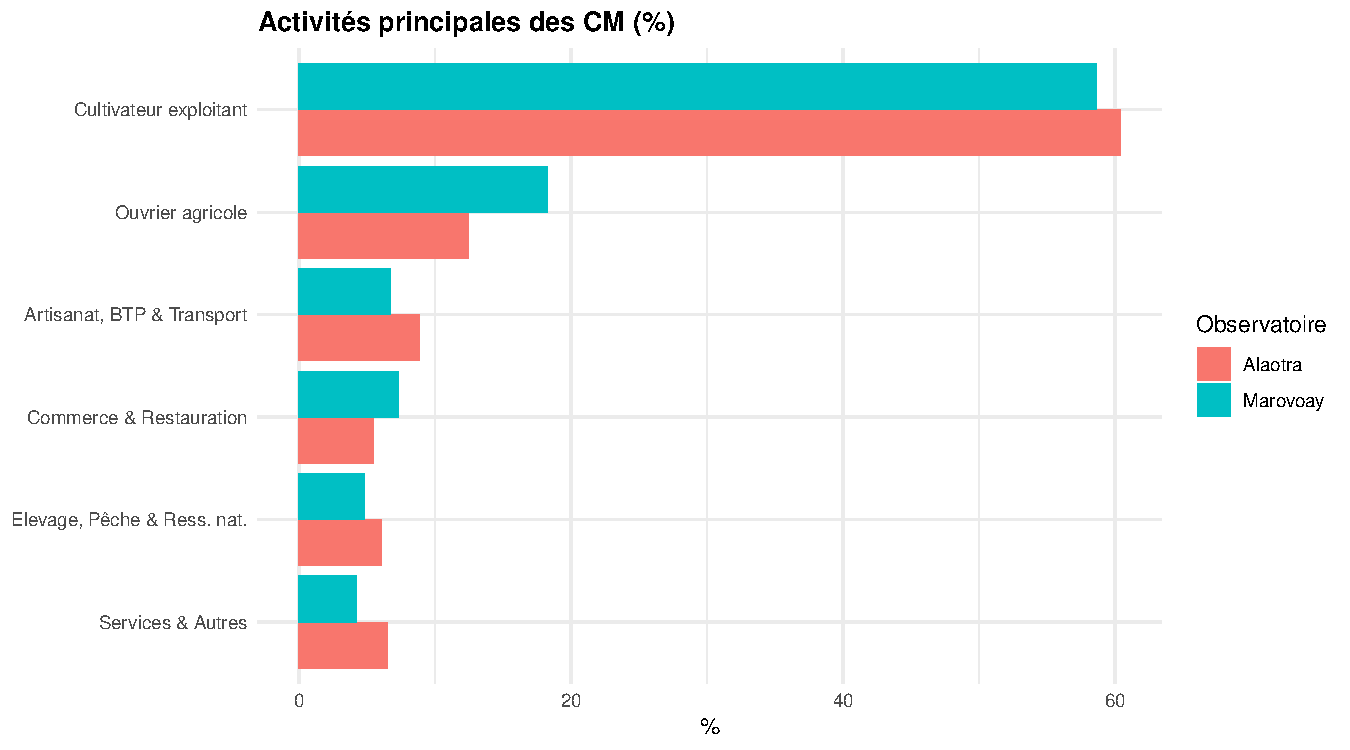
\includegraphics[keepaspectratio]{test_layout_files/figure-pdf/fig-test-bar-1.pdf}}

}

\caption{\label{fig-test-bar}}

\end{figure}%

\chapter{Test 8: Figure --- faceted bar chart by
sex}\label{test-8-figure-faceted-bar-chart-by-sex}

\begin{figure}

\centering{

\pandocbounded{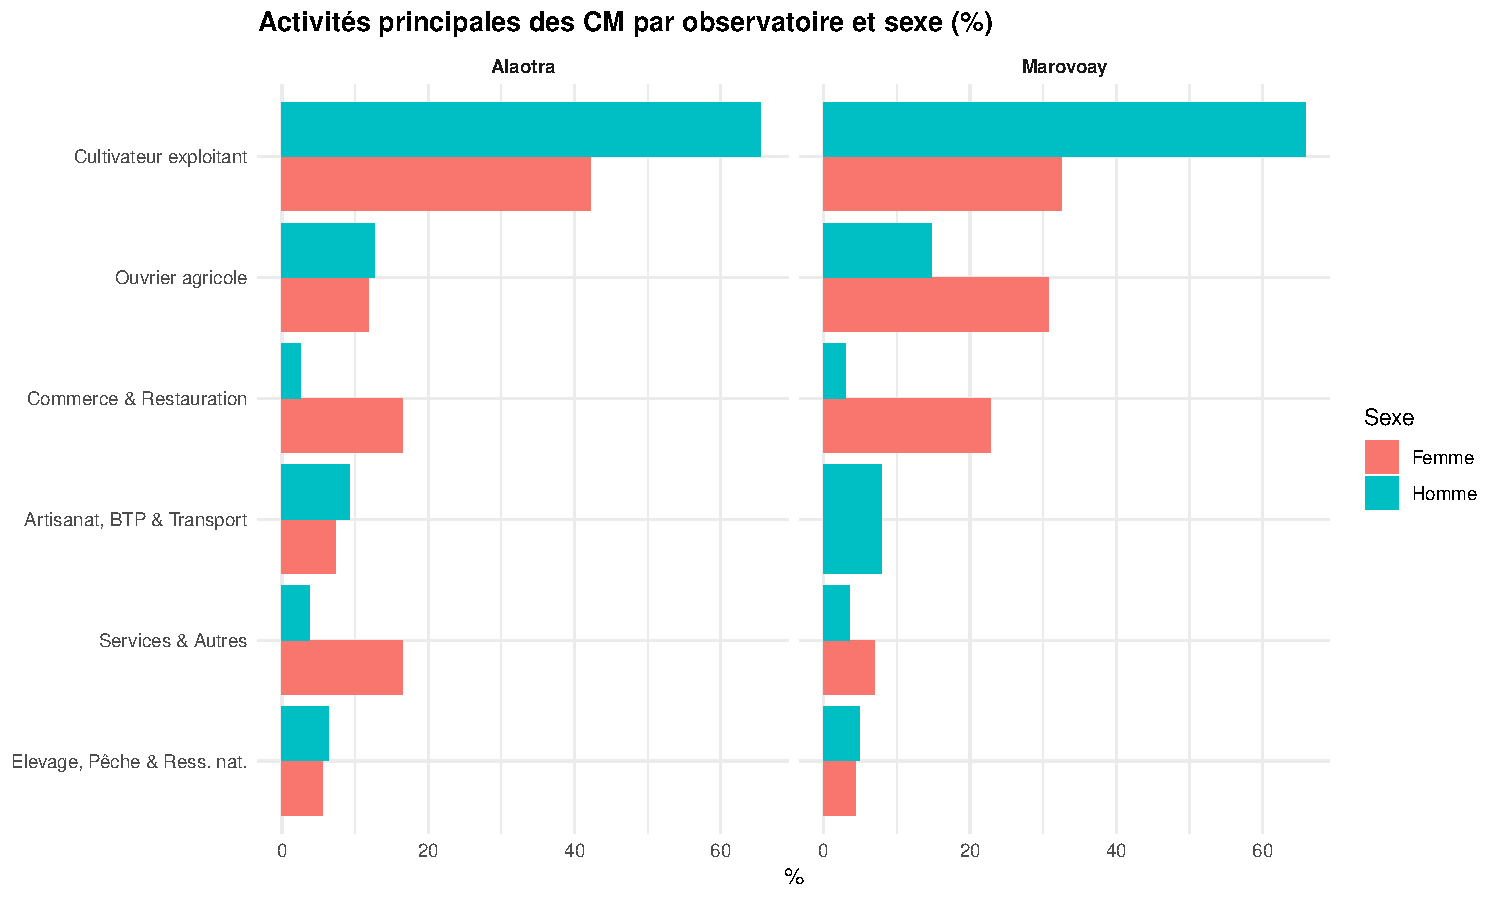
\includegraphics[keepaspectratio]{test_layout_files/figure-pdf/fig-test-faceted-1.pdf}}

}

\caption{\label{fig-test-faceted}}

\end{figure}%

\chapter{Test 9: Figure --- pyramide des
âges}\label{test-9-figure-pyramide-des-uxe2ges}

\begin{figure}

\centering{

\pandocbounded{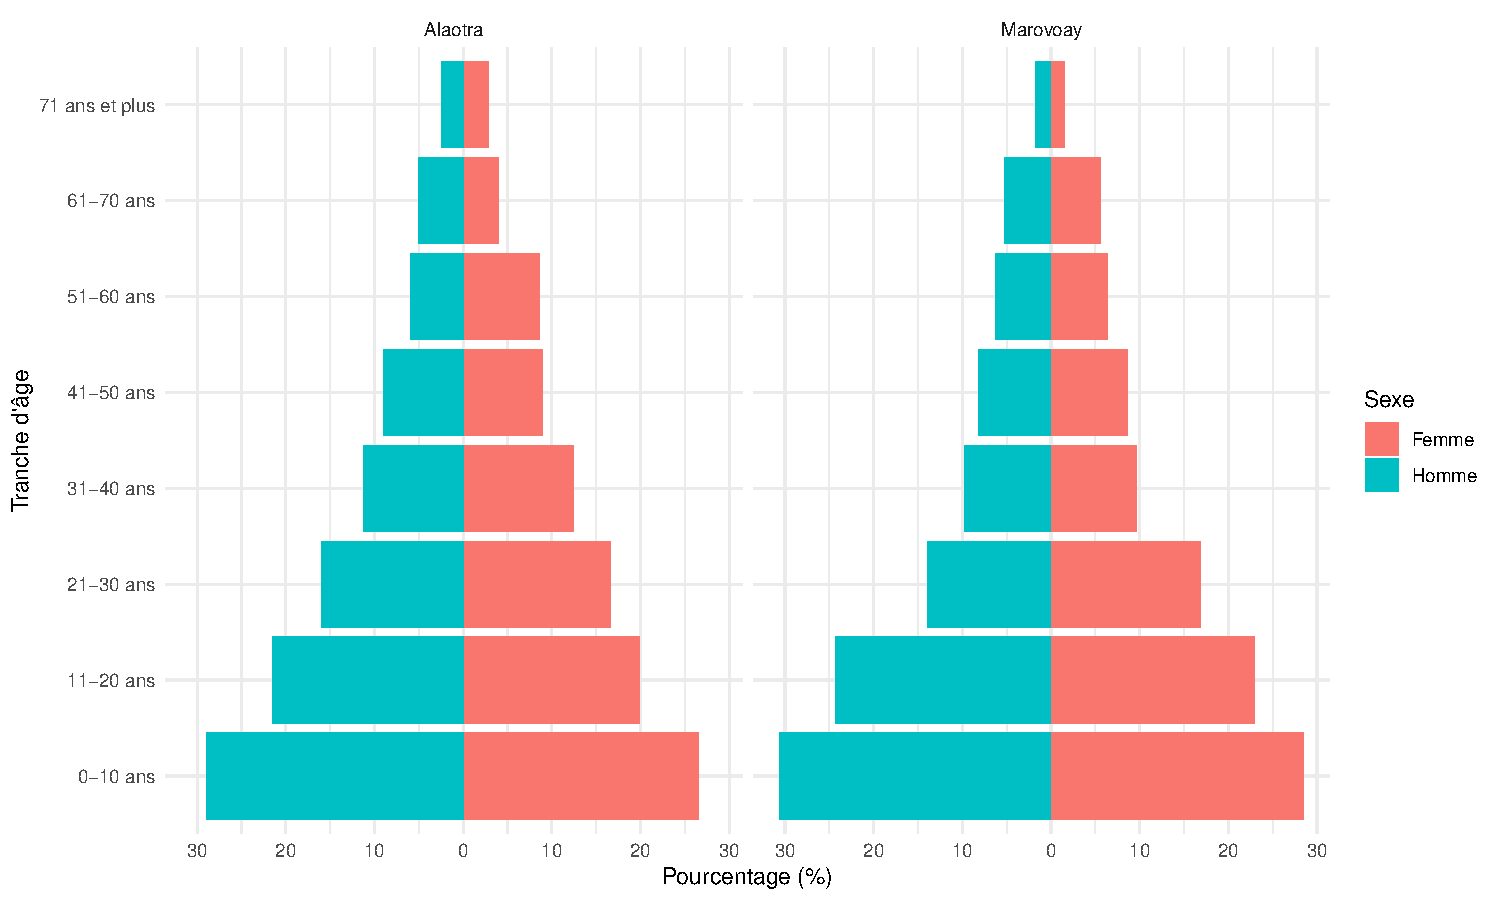
\includegraphics[keepaspectratio]{test_layout_files/figure-pdf/fig-test-pyramid-1.pdf}}

}

\caption{\label{fig-test-pyramid}}

\end{figure}%

\chapter{Test 10: CM characteristics combined
table}\label{test-10-cm-characteristics-combined-table}

\begin{longtable}[]{@{}lll@{}}

\caption{\label{tbl-test-cm-chars}}

\tabularnewline

\toprule\noalign{}
\multicolumn{3}{@{}c@{}}{%
Caractéristiques des chefs de ménage} \\
Catégorie & Alaotra & Marovoay \\
\midrule\noalign{}
\endhead
\midrule\noalign{}
\multicolumn{3}{@{}l@{}}{%
{\textbf{Source : Enquête auprès des OR 2025}}} \\
\bottomrule\noalign{}
\endlastfoot
\multicolumn{3}{@{}l@{}}{%
Sexe} \\
Femme & 110 (21.7\%) & 114 (22\%) \\
Homme & 397 (78.3\%) & 405 (78\%) \\
\multicolumn{3}{@{}l@{}}{%
Âge} \\
Médiane & 43 & 45 \\
Moyenne & 45 & 46 \\
Minimum & 16 & 18 \\
Maximum & 90 & 96 \\

\end{longtable}




\end{document}
